
\documentclass{article}

% Recommended, but optional, packages for figures and better typesetting:
\usepackage{microtype}
\usepackage{graphicx}
\usepackage{subcaption}
\usepackage{colortbl}
\usepackage{booktabs} % for professional tables

% hyperref makes hyperlinks in the resulting PDF.
% If your build breaks (sometimes temporarily if a hyperlink spans a page)
% please comment out the following usepackage line and replace
% \usepackage{icml2026} with \usepackage[nohyperref]{icml2026} above.
\usepackage{hyperref}


% Attempt to make hyperref and algorithmic work together better:
\newcommand{\theHalgorithm}{\arabic{algorithm}}

\usepackage{icml2026}

\usepackage{graphicx}

\usepackage{amsmath}
\usepackage{amssymb}
\usepackage{mathtools}
\usepackage{amsthm}
\usepackage{xspace}
\usepackage[textsize=tiny]{todonotes}
\usepackage[capitalize,noabbrev]{cleveref}
%%%%%%%%%%%%%%%%%%%%%%%%%%%%%%%%
% THEOREMS
%%%%%%%%%%%%%%%%%%%%%%%%%%%%%%%%
\theoremstyle{plain}
\newtheorem{theorem}{Theorem}[section]
\newtheorem{proposition}[theorem]{Proposition}
\newtheorem{lemma}[theorem]{Lemma}
\newtheorem{corollary}[theorem]{Corollary}
\theoremstyle{definition}
\newtheorem{definition}[theorem]{Definition}
\newtheorem{assumption}[theorem]{Assumption}
\theoremstyle{remark}
\newtheorem{remark}[theorem]{Remark}

% Optional math commands from https://github.com/goodfeli/dlbook_notation.
%\input{math_commands.tex}
\newcommand{\ours}{{\sc NeSyS}\xspace}
\usepackage[inline]{enumitem}
\usepackage{newtxtext,newtxmath}
\usepackage{tcolorbox}
\tcbuselibrary{breakable}


\icmltitlerunning{Neuro-Symbolic Synergy for Interactive World Modeling}

\begin{document}
\twocolumn[
  \icmltitle{Neuro-Symbolic Synergy for Interactive World Modeling}

  % It is OKAY to include author information, even for blind submissions: the
  % style file will automatically remove it for you unless you've provided
  % the [accepted] option to the icml2026 package.

  % List of affiliations: The first argument should be a (short) identifier you
  % will use later to specify author affiliations Academic affiliations
  % should list Department, University, City, Region, Country Industry
  % affiliations should list Company, City, Region, Country

  % You can specify symbols, otherwise they are numbered in order. Ideally, you
  % should not use this facility. Affiliations will be numbered in order of
  % appearance and this is the preferred way.
  \icmlsetsymbol{equal}{*}

  \begin{icmlauthorlist}\icmlauthor{Anonymous}{anon}\end{icmlauthorlist}

  \icmlaffiliation{anon}{Anonymous Institution}
  
  
  
  

  \icmlcorrespondingauthor{Anonymous}{anonymous@anonymous.invalid}
  

  % You may provide any keywords that you find helpful for describing your
  % paper; these are used to populate the "keywords" metadata in the PDF but
  % will not be shown in the document
  \icmlkeywords{World modeling, Neurosymbolic, Language Model}

  \vskip 0.3in
]

\printAffiliationsAndNotice{}

\begin{abstract}
Large language models (LLMs) exhibit strong general-purpose reasoning capabilities, yet they frequently hallucinate when used as world models (WMs), where strict compliance with deterministic transition rules—particularly in corner cases—is essential. In contrast, Symbolic WMs provide logical consistency but lack semantic expressivity. To bridge this gap, we propose \emph{Neuro-Symbolic Synergy} (\ours), a framework that integrates the probabilistic semantic priors of LLMs with executable symbolic rules to achieve both expressivity and robustness. \ours alternates training between the two models using trajectories inadequately explained by the other.
Unlike rule-based prompting, the symbolic WM directly constrains the LLM by modifying its output probability distribution. The neural WM is fine-tuned only on trajectories not covered by symbolic rules, reducing training data by 50\% without loss of accuracy.
Extensive experiments on three distinct interactive environments, i.e., ScienceWorld, Webshop, and Plancraft, demonstrate \ours's consistent advantages over baselines in both WM prediction accuracy and data efficiency. 

Our models and code are available at \url{https://github.com/tianyi-lab/NeSyS}.
\end{abstract}

\begin{figure}[ht]
    \centering
    \includegraphics[width=\columnwidth]{images/cover.png}
    \caption{An example of the world modeling task. Given the current belief state and the agent's next action, the world model needs to predict the next state. Both a neural world model (LLM) and a symbolic world model fail to answer the question by themselves. We propose to combine the two world models by viewing the symbolic scores as an energy term that modifies the probability distribution of the neural world model.}
    \label{fig:cover}
\end{figure}

\section{Introduction} \label{sec:intro}
Large language models (LLMs) have recently emerged as strong general-purpose world models (WMs) for sequential decision-making problems~\citep{yang2024evaluating}. With broad world knowledge and powerful general reasoning capabilities, they perform competitively across a wide range of tasks. However, LLMs often struggle to produce accurate predictions in domains with structured observations and well-defined dynamics, such as games and web environments~\citep{levy2025worldllm, chae2024web}. In particular, despite their strong performance in stochastic settings, they frequently fail in deterministic scenarios that require strict adherence to transition rules and constraints~\citep{duan2024gtbench}. Although extensive domain-specific fine-tuning can partially mitigate these issues, the inherently probabilistic nature of LLMs makes strict adherence to hard constraints difficult to guarantee. Moreover, their reliance on statistical learning limits their ability to reliably capture rare corner cases and long-tail behaviors. 
% causes LLMs to occasionally violate hard constraints and to poorly capture rare but critical long-tailed behaviors. 

To address the shortcomings of WMs that rely solely on neural networks, a parallel line of work focuses on learning explicit symbolic WMs~\citep{agravante2023learning,liang2024visualpredicator}. By enforcing hard rules and deterministic transition structures, such models naturally avoid constraint violations and long-horizon inconsistencies. However, their expressiveness is fundamentally limited: they struggle to generalize to real-world interactive environments whose dynamics are complex, high-dimensional, stochastic, or too underspecified to admit a tractable rule-based formulation. This limitation becomes particularly severe in natural-language-driven environments, where predicting the exact next state is often infeasible without leveraging the rich semantic priors embedded in large language models.

These limitations suggest that neither purely neural WMs nor purely symbolic WMs are sufficient on their own, motivating the need for \textbf{neuro-symbolic synergy} (\ours) in world modeling. \Cref{fig:cover} illustrates this motivation with an example in which \ours correctly answers a question that both approaches fail to resolve on their own. A variety of neuro-symbolic approaches have been explored. For instance, WALL-E~\citep{zhou2024wall,zhou2025wall} injects symbolic rules into the decision process by prepending them to the LLM’s input context, thereby constraining next-state prediction implicitly. While effective when paired with large, instruction-tuned models, this strategy does not reliably transfer to smaller or more heavily fine-tuned models. In practice, such models frequently ignore or override injected instructions, limiting the robustness and scalability of context-based rule enforcement.

In contrast, we propose to \textbf{directly modify the probability distribution of the LLM with symbolic rules implemented by Python functions}. This design yields two key advantages. First, the LLM is not required to follow additional instructions, eliminating any reliance on instruction-following quality or prompt sensitivity. Second, rules can be evaluated efficiently and locally (without additional inference on LLMs) by inspecting the probabilities of a small set of candidate answers annotated with ground-truth correctness, enabling rapid feedback and making rule learning substantially more sample-efficient than injecting rules into LLM context.

Furthermore, we observe that extensive fine-tuning of the neural WM is often unnecessary, as many failure cases can be resolved through simple and generalizable rules. Based on this insight, we introduce \textbf{rule-guided data selection}, which filters out training examples whose dynamics are already captured by learned rules, thereby reducing training redundancy. Empirically, it halves the training data while maintaining comparable performance, highlighting the practical efficiency of explicit neuro-symbolic synergy.

We examine the world modeling capabilities by a suite of benchmarks spanning three diverse and widely-studied environments: ScienceWorld~\citep{scienceworld2022}, Webshop~\citep{yao2022webshop} and Plancraft~\citep{dagan2024Plancraft}. They capture challenges in common-sense physical reasoning, real-world web interaction, and structured game dynamics, respectively. Across all three, we demonstrate that \ours consistently outperforms baselines on different choices of backbone LLMs, highlighting both its effectiveness and robustness. 

In summary, this work makes the following contributions:
\begin{itemize}
    \item We introduce \emph{Neuro-Symbolic Synergy} (\ours), a framework that integrates LLM-based world models with symbolic rules by directly enforcing hard constraints through probability-level modification of LLM outputs.
    \item We introduce a complementary training paradigm for neural and symbolic world models, where each model is trained only on data regimes not handled by the other, substantially reducing finetuning data requirements without sacrificing performance.
    %We train a neural WM and a symbolic WM in a complementary manner, and let each training focus on data that cannot be covered by the other. This strategy substantially reduces finetuning data without compromising performance. 
    % rule-guided data selection, a data-efficient training strategy that substantially reduces fine-tuning requirements without sacrificing performance.
    \item We empirically demonstrate that \ours achieves consistent performance improvements across diverse interactive environments and model scales.
\end{itemize}

\section{Related Works}
\paragraph{Neuro-symbolic world models.} %The concept of a World Model (WM) has evolved significantly, transitioning from classical reinforcement learning frameworks~\citep{ha2018world} to modern large-scale applications. 
%Recently, Large Language Models (LLMs) have been leveraged as general-purpose simulators for sequential decision-making~\citep{yang2024evaluating,levy2025worldllm}. 
%However, 
To mitigate inherent limitations of pure neural models—such as hallucination—neuro-symbolic world models have emerged as a promising paradigm~\citep{cano2025neurosymbolic, sehgal2023neurosymbolic, balloch2023neuro}. In complex, text-rich environments, existing methods often employ semantic parsers~\citep{agravante2023learning} or VLMs~\citep{liang2024visualpredicator} to translate environment dynamics into symbolic rules. To better synergize neural and symbolic components, recent works have explored enhancing LLM prompts with symbolic constraints: \citet{de2025neurosymbolic} utilize knowledge graphs to prompt the model with structured knowledge, while WALL-E~\citep{zhou2024wall,zhou2025wall} prepends symbolic rules to the LLM’s context. Nevertheless, such prompt engineering approaches rely heavily on the model's instruction-following capabilities. To address this reliance, our work proposes to directly modify the LLM's output probability distribution using executable Python rules.

\paragraph{Training data selection.} Data selection is critical for optimizing the performance of fine-tuned LLMs while minimizing computational costs~\citep{zhou2023lima}. While recent literature has explored rule-based methods to identify high-quality training subsets~\citep{li2024rule}, our approach diverges in its objective. Instead of filtering for general data quality% to enhance the model in isolation, we utilize rules to identify instances that are difficult for symbolic rules to solve. 
, we aim to maximize the complementary strengths of the neural model and the symbolic components by selecting instances that are difficult for symbolic rules to solve.
%, thereby improving the overall system performance.

\paragraph{Constrained decoding and logit manipulation.} Constrained decoding is a well-established technique for forcing LLM outputs to adhere to specific formats~\citep{willard2023efficient,beurer2024guiding}. While traditional constrained decoding focuses on syntactic correctness (e.g., generating valid JSON), recent works have begun exploring semantic and logical constraints~\citep{wu2024self,ma2025logically}. \ours extends this line of research by using symbolic evaluations as an energy-based shifting factor in the probability landscape. %Unlike "black-box" constrained decoders that rely on rejected sampling or prefix-trees, our framework uses locally evaluable Python functions to re-rank candidate transitions, making it computationally efficient and agnostic to the underlying LLM’s instruction-following capabilities.

\section{Problem Setting}\label{sec:problem}
We study sequential decision-making problems in a partially observable Markov decision process (POMDP). At step $t$, the agent needs to do action $a_t$ based on the current belief state $b_t$. It will then receive the next state $s_{t+1}$ and a reward $r_t$ from the environment.  \footnote{We do not distinguish observation and state here. See \cref{app:pomdp} for a rigorous definition.}
% $\mathcal{M} = (S, A, T, R, \Omega, O)$, where $S$ denotes the latent state space, $A$ the action space,
% $T : S \times A \to \Delta(S)$ the transition kernel, $R : S \times A \to \mathbb{R}$ the reward function,
% $\Omega$ the observation space, and $O : S \times A \to \Delta(\Omega)$ the observation kernel. Both actions $a_t \in A$ and observations $\omega_t \in \Omega$ are represented as natural-language strings,
% reflecting the interactive environments considered in this work.

A \textbf{world model} is defined as a predictive model that estimates the next state $s_{t+1}$ and reward $r_t$ conditioned on the current belief state $b_t$ and action $a_t$. Following prior LLM-based agent work, we approximate the belief state by a textual context constructed from the task description $g$ and a truncated history of recent observations, actions, and rewards that fit within the model’s context window.

\section{Method}\label{sec:method}
Our framework consists of two world models (WM): Neural WM and Symbolic WM. Neural WM is in the form of an LLM, while Symbolic WM is a weighted set of Python rules. %Either WM can score candidate $(s_t,r_t)$ pairs on its own\footnote{Candidates can be generated by Neural WM or provided a priori.}, but rather than treating the two components as separate black box scorers, our approach dynamically integrates them during inference and iteratively refines them during training. 

\subsection{Framework Overview}
\begin{figure}[ht]
        \centering
        \includegraphics[width=0.8\linewidth]{images/inference.png}
        \caption{\textbf{Overview of \ours}. It consists of two world models: Neural WM and Symbolic WM. They are implemented as an LLM $\theta$ with likelihood function $P_\theta$ and a weighted rule set $\mathcal{F}$, respectively. Neural WM generates $K$ candidates of the next state and reward pairs if there is no provided choices. The likelihood $p_i$ for each candidate is computed. Symbolic WM aggregates the score $e_{ij}$ produced by each rule $f_j$. We then modify the likelihood $p_i$ with the score by Symbolic WM, and choose the candidate with the largest modified likelihood $\tilde{p}_i$. For simplicity, the conditional $b_t$ and $a_t$ are omitted from the parameters of $P_\theta$ and $f_j$.}
        \label{fig:inference}
\end{figure}

As mentioned in \cref{sec:intro}, the main idea of our strategy is to directly modify the probability distribution of Neural WM, i.e., LLM, with the symbolic rules learned by Symbolic WM. Given current belief state $b_t$ and action $a_t$, we aim to select the optimal next-step state and reward. The whole inference pipeline is illustrated in \cref{fig:inference}.

% To align each WM with its comparative advantage, we employ a lightweight \text{router} (an XGBClassifier) to dynamically determine whether to query the neural module only, the symbolic module only, or both. During the training stage (that we will discuss in \cref{sec:training} later), we will iteratively refine the neural and symbolic modules, and will naturally hold different versions of them. As a bonus, we also allow the router to choose a module from previous versions.

On the left side, Neural WM computes the likelihood ${p_i}$ for candidate next state $s_{t+1}^{i}$ and reward $r_t^{i}$. The $K$ candidates are either provided or generated by Neural WM itself. 

On the right side, Symbolic WM is implemented as a weighted set of executable Python functions $\mathcal{F}=\{(f_j, w_j)\}_{j=1}^m$, where $f_j\!:\!(b_t,a_t,s_{t+1},r_t)\mapsto[-1,1]$. Each rule produces a score $e_{ij} \in [-1, 1]$ indicating how likely the candidate $(s_{t+1}^i,r_t^i)$ is correct under this specific rule. Rules are typically inactive and output zero, but become active only when specific conditions are met (e.g., a particular action is taken or a relevant keyword appears in the belief state). We aggregate these logical judgments into a scalar shifting factor $E_i$ using learned rule weights $w_j$: $$E_i = \sum_{j=1}^m w_j e_{ij}$$

We combine these signals by treating the symbolic score as an energy term that modifies the neural likelihood $p_i$. The modified likelihood $\tilde{p}_i$ is computed as 
\begin{equation*}
\tilde{p}_i = p_i\exp(\gamma E_i),
\end{equation*}
where the scaling factor $\gamma$ is a global hyperparameter. In our experiments, it's set as either $1$ (no scaling) or the largest gap of log likelihood between candidates. 

We then select the candidate with the largest $\tilde{p}_i$. This formulation allows Symbolic WM to enforce hard constraints via a negative $E_i$ or boost logical consistencies via a positive $E_i$, effectively reshaping the probability landscape of the LLM.

\subsection{Training Pipeline}\label{sec:training}
\begin{figure}[ht]
        \centering
        \includegraphics[width=\linewidth]{images/training_pipeline.png}
        \caption{\textbf{Training pipeline of \ours}. It consists of two phases. In Phase 1 (Initialization), we initialize Neural WM with a pretrained LLM. We evaluate it on the development set to separate common sense from task-specific knowledge, generating rules for the latter to initialize Symbolic WM. In Phase 2 (Reciprocal Refinement), we use Symbolic WM to perform rule-guided data selection on the training set by filtering out simple cases. The remaining ``hard'' data are used to fine-tune Neural WM. Symbolic WM is then refined by addressing long-tailed cases where the updated Neural WM still fails. Legend is in the lower left corner. Weight optimization for Symbolic WM is omitted for clarity.}
        \label{fig:training}
\end{figure}
As illustrated in \cref{fig:training}, our training pipeline consists of two phases: Initialization and Reciprocal Refinement. The pipeline iteratively filters out training / development samples that can be covered by the current framework, and improve the two WMs based on the errors of each other. This design ensures that the two WMs evolve complementarily rather than redundantly.

\subsubsection{Phase 1: Initialization.}
\paragraph{Neural WM.}
We initialize Neural WM using a pretrained LLM. By evaluating this model on the development set, we can separate questions that can be solved with general common sense knowledge (correct samples) from those that require task-specific knowledge (incorrect samples). 

\paragraph{Symbolic WM.}
We aim to capture task-specific deterministic dynamics that Neural WM misses via explicit rules. The rules are induced via an automated debugging loop:
\begin{enumerate}
\item \textbf{Error clustering:} We identify mistakes made by the initialized Neural WM on a development set. These are clustered by syntactic and semantic similarity (details in \cref{app:clustering}) to identify systematic failure modes.
\item \textbf{Rule generation:} For each cluster, we prompt \texttt{gpt-5-mini} to write a Python function that corrects the specific error while generalizing to similar cases.
\item \textbf{Verification \& weighting:} A rule is added to $\mathcal{F}$ only if the accuracy of \ours on the development set is improved with the update $\mathcal{F}$. We perform up to 3 reflection iterations with \texttt{gpt-5-mini} for failed rules. We initialize the scalar weights uniformly as $w_j=1$.
%Finally, we learn scalar weights $w_j$ via coordinate descent to maximize the performance of \ours on the development set.
\end{enumerate}

\subsubsection{Phase 2: Reciprocal Refinement.}
\paragraph{Neural WM.}
A key insight of our work is that fine-tuning a model on behaviors already captured by explicit rules is computationally wasteful and potentially redundant. To address this, we introduce \textbf{rule-guided data selection}. 

We evaluate the training trajectories using our initialized rule set $\mathcal{F}$. For each step, we compute $k$ to be the number of rules in $\mathcal{F}$ that reports a non-zero score on it. The steps with smaller $k$ is harder to predict by the Symbolic WM alone and vice versa. We first collect all the steps with $k=0$ and sample from the remaining steps with probability proportional to $\frac{1}{k}$ so that harder steps are sampled more frequently. Neural WM is then fine-tuned only on the sampled examples. This focuses the Neural WM's capacity on capturing complex, intuitive dynamics that are difficult to formalize as code. In practice, we find this strategy can discard about half of training data while maintaining or improving performance.

%We aim to filter out steps where Symbolic WM already strongly predicts the outcome. Each training step $i$ is assigned a sampling weight $\frac{1}{k}$, where $k$ represents the number of rules that report a non-zero score on this step. The steps where $k=0$ are selected with probability $1$, while about 25\% of the rest are selected with a weighted sampling. A larger $k$ indicates that this step can likely be predicted with Symbolic WM.


\paragraph{Symbolic WM.}
Following refinement of Neural WM, rules that were useful for a weaker Neural WM might now negatively impact the performance. We first apply a cleaning pass: any rule that has a negative impact on the performance of Neural WM is discarded. We then add more rules by repeating the clustering and synthesis process described in Phase 1 to cover any new residual errors.

Finally, in order to enhance the performance of \ours, we learn scalar weights $w_j$ via coordinate descent on the development set.

% \subsubsection{Phase 3: Router training.}
% To exploit the strengths of each module, we train a lightweight router to predict the necessity of each module. It can also choose to use modules from phase 1 or phase 2. The router takes input features such as task metadata, input length, and rule activation scores. It learns to choose the module pair that can maximize the margin of perplexities between the correct answer and the best distractor. See \cref{app:router} for router implementation details.
\begin{table*}[ht]
  \caption{World modeling accuracy on ScienceWorld. \textbf{Bold} numbers highlight the best performance for each backbone model. }
  \label{tab:wm_science_world}
  \centering
  \begin{tabular}{lcccccccc}
    \toprule
    \cmidrule(r){1-2}
    World Model     & Matter & Chem. & Class. & Biology & Forces & Meas. & Elec. & Avg.\\
    \midrule
    \rowcolor{gray!15}
    \multicolumn{9}{c}{\bf Baseline Models} \\
    \midrule
    Llama3.1-8B & 36.1 & 29.4 & 68.8 & 42.7 & 38.9 & 52.5 & 33.9 & 44.4 \\
    Qwen3-8B & 38.9 & 31.4 & 65.0 & 43.3 & 66.7 & 45.8 & 40.7 & 46.5 \\
    Qwen3-14B & 45.8 & 43.1 & 68.8 & 46.5 & 64.9 & 47.5 & 49.2 & 51.2 \\
    Phi-4-mini & 38.9 & 39.2 & 63.8 & 50.3 & 50.0 & 40.7 & 33.9 & 46.7 \\
    GPT-oss-20B &34.7& 49.0& 48.8& 47.7& 40.6& 33.9& 25.4& 41.2\\
    GPT-5-mini & 45.8 & 51.0 & 72.5 & 52.2 & 72.2 & 50.8 & 50.8 & 55.4\\
    \midrule
    \rowcolor{gray!15}
    \multicolumn{9}{c}{\bf Llama3.2-1B} \\
    \midrule
    SFT (100\% data)& 37.5 & 64.7& 81.3& 68.8& 80.6 & \textbf{54.2} & \textbf{62.7} & 64.4\\
    \midrule
    Neural WM (Phase 1) & 27.8 & 17.7 & 42.5 & 39.5 & 44.4 & 27.1 & 15.3 & 32.3\\
    Symbolic WM (Phase 1) & 33.3 & 39.2 & 58.8 & 56.7 & 41.7 & 30.5 & 47.5 & 46.9\\
    \ours\ (Phase 1) & 43.1 & 27.5 & 61.3 & 58.6 & 50.0 & 42.4 & 37.3 & 48.8\\
    \midrule
    Neural WM (Phase 2) & 37.5 & \textbf{66.7} & 71.3 & 70.1 & 77.8 & 47.5 & 55.9 & 61.7\\
    Symbolic WM (Phase 2) & 45.8 & 41.2 & 78.8 & 56.7 & 41.7 & 45.8 & 55.9 & 54.7\\
    \ours~(ours, 45\% data\footnotemark) & \textbf{47.2} & 64.7 & \textbf{88.8} & \textbf{73.3} & \textbf{91.7} & 50.9 & 59.3 & \textbf{68.3}\\
    % \midrule
    % \rowcolor{gray!15}
    % % $\text{\ours}_\text{oracle}$ 
    % Oracle & 65.3 & 82.4 & 83.8 & 89.8 & 97.2 & 67.8 & 71.2 & 80.5\\  
    % % $\text{\ours}$ 
    % \ours~(ours) & \textbf{47.2} &\textbf{66.7} & 73.8 & \textbf{73.2} & \textbf{91.7} & 49.2 & 59.3 & \textbf{66.0}\\
    \midrule
    \rowcolor{gray!15}
    \multicolumn{9}{c}{\bf Qwen3-4B} \\
    \midrule
    SFT (100\% data) & 48.6 & \textbf{66.7} & \textbf{91.3} & 68.8 & \textbf{100.0} & \textbf{59.3} & 50.8 & 68.3 \\
    \midrule
    Neural WM (Phase 1) & 38.9 & 35.3 & 63.8 & 43.3 & 63.9 & 42.4 & 47.5 & 46.9 \\
    Symbolic WM (Phase 1) & 38.9 & 47.1 & 52.5 & 61.2 & 41.7 & 33.9 & 54.2 & 50.0 \\
    \ours\ (Phase 1) 
    & \textbf{52.8} & 43.1 & 68.8 & 62.4 & 63.9 & 55.9 & 54.2 & 58.6\\
    \midrule
    Neural WM (Phase 2) & 50.0 & 58.8 & \textbf{91.3} & 66.9 & 94.4 & \textbf{59.3} & \textbf{66.1} & 68.5\\
    Symbolic WM (Phase 2) & 43.1 & 58.8 & 68.8 & 62.4 & 75.0 & 44.1 & 55.9 & 58.4 \\
    \ours~(ours, 45\% data) & 50.0 & 60.8 & 88.8 & \textbf{75.8} & 94.4 & \textbf{59.3} & \textbf{66.1} & \textbf{71.0}\\
    % \midrule
    % \rowcolor{gray!15}
    % % $\text{\ours}_\text{oracle}$ 
    % Oracle
    % & 76.4 & 76.5 & 96.3 & 88.5 & 100.0 & 76.3 & 81.4 & 85.4\\
    % % $\text{\ours}_\text{router}$ & 73.3 & 49.0 & 76.3 & 66.1 & 83.3 & 56.9 & 49.2 & 65.2\\
    % \ours~(ours) & \textbf{55.6} & 64.7 & 90.0 & \textbf{77.7} & 94.4 & \textbf{59.3} & \textbf{67.8} & \textbf{73.2} \\
    \bottomrule
  \end{tabular}
\end{table*}
\section{Experiments} \label{sec:exp}
\subsection{Experiment Setup} \label{sec:exp_setup}
\paragraph{Environments.} We evaluate our methods on three diverse environments: ScienceWorld~\citep{scienceworld2022}, Webshop~\citep{yao2022webshop} and Plancraft~\citep{dagan2024Plancraft}, which respectively capture challenges in common-sense physical reasoning, real-world web interaction, and structured game dynamics. Based on these environments, we create multiple-choice questions for both developing and testing. Details can be found in \cref{app:data-collection}.
% \begin{itemize}
%     \item \textbf{ScienceWorld}~\citep{scienceworld2022}: ScienceWorld is an environment for agents to navigate through rooms and perform tasks aligned with a standardized elementary science curriculum. World models need to perform common-sense reasoning and understand different scientific rules in each task.
%     \item \textbf{Webshop}~\citep{yao2022webshop}: Webshop is an e-commerce website environment to test the comprehensive ability of agents in complicated and noisy real-world dynamics. It requires the agent to navigate webpages, search and purchase items that satisfy particular requirements. World models need to infer possible search results, descriptions of the items, understand the layout of webpages and effects of each button, and judge whether the purchased item meets the requirement. 
%     \item \textbf{Plancraft}~\citep{dagan2024Plancraft}: Plancraft is a Minecraft-based environment that constrains interaction to the Minecraft crafting GUI, requiring agents to use items in the backpack to craft certain items. World models need to know the crafting recipes (or infer them from common sense) and understand the general crafting rules of the game.
% \end{itemize} 
\paragraph{Models and baselines.} We evaluate the performance of Llama3.2-1B instruct version~\citep{grattafiori2024llama} and Qwen3-4B~\citep{qwen2, qwen2.5} as the backbone of the neural world model. The rules for the symbolic part are generated by \texttt{gpt-5-mini}~\citep{singh2025openai}. We compare against multiple strong open-source models along with proprietary models, including Llama3.1-8B instruct version, Qwen3-8B/14B, Phi-4-mini~\citep{abouelenin2025phi}, GPT-oss-20B~\citep{agarwal2025gpt} and GPT-5-mini. We also consider the natural baseline that fine-tunes the backbone LLM on the full training data. Additionally, we provide a detailed ablation analysis covering performance of each single world model and \ours across both Phase 1 and Phase 2. For fair comparison, we also learn a weight for \ours in Phase 1.
%\paragraph{Benchmark creation.} We create the benchmarks based on the official expert trajectories provided by the environment. For clearer metrics, we formulate the dev/test sets as multiple-choice questions by randomly select positions in the trajectories and generate distractors with \texttt{Llama-3.2-1B-instruct}. Details can be found in \cref{app:data-collection}.

\subsection{ScienceWorld}\label{sec:scienceworld}
To access the common-sense reasoning abilities of world models, we evaluate our methods on ScienceWorld, where the models need to navigate through a series of rooms and perform tasks aligned with a standardized elementary science curriculum. The tasks are divided into 7 different topics, including matter, chemistry, classification, biology, forces, measurement and electricity. We report accuracy on each topic along with the average accuracy in \cref{tab:wm_science_world}.
\begin{table*}[ht]
  \caption{
  World modeling accuracy on Webshop. \textbf{Bold} numbers highlight the best performance for each backbone model.
  % World modeling task performance on Webshop. The evaluation metric is accuracy. The oracle method is marked as grey as it uses test set information. Bold numbers indicate best performance for that backbone model, excluding the oracle method.
  }
  \label{tab:wm_webshop}
  \centering
  \begin{tabular}{lccccccc}
    \toprule
    \cmidrule(r){1-2}
    World Model & Search & Layout & Detail & Decision & Page Change & Other & Avg.\\
    \midrule
    \rowcolor{gray!15}
    \multicolumn{8}{c}{\bf Baseline Models} \\
    \midrule
    Llama3.1-8B & 0.0 & 2.9 & 10.2 & 50.0 & 2.7 & 29.1 & 28.9\\
    Qwen3-8B & 0.0 & 0.0 & 14.3 & 39.5 & 2.7 & 32.6 & 25.1\\
    Qwen3-14B & 0.0 & 2.9 & 12.2 & 46.2 & 2.7 & 31.9 & 27.9\\
    Phi-4-mini & 0.0 & 0.0 & 4.1 & 50.0 & 2.7 & 11.3 & 24.9\\
    GPT-oss-20B & 0.0 & 0.0 & 16.3 & 50.0 & 5.4 & 0.7 & 24.0\\
    GPT-5-mini & 89.4 & 94.1 & 81.6 & 66.9 & 94.6 & 96.5 & 81.4\\
    \midrule
    \rowcolor{gray!15}
    \multicolumn{8}{c}{\bf Llama3.2-1B} \\
    \midrule
    SFT (100\% data) & 0.0 & 58.8 & 20.4 & 50.0 & 10.7 & \textbf{100.0} & 47.5\\
    \midrule
    Neural WM (Phase 1) & 0.0 & 0.0 & 0.0 & 50.0 & 0.9 & 0.7 & 22.2\\
    Symbolic WM (Phase 1) & \textbf{100.0} & 23.5 & 81.6 & \textbf{83.8} & 75.0 & 96.5 & 83.4\\
    \ours\ (Phase 1) & 98.5 & 2.9 & 73.5 & \textbf{83.8} & 71.4 & 95.0 & 80.9\\
    \midrule
    Neural WM (Phase 2) & 0.0 & 52.9 & 19.2 & 50.0 & 12.4 & \textbf{100.0} & 45.9\\
    Symbolic WM (Phase 2) & \textbf{100.0} & 88.2 & \textbf{98.0} & \textbf{83.8} & \textbf{100.0} & 96.5 & 91.5\\
    \ours~(ours, 60\% data) & \textbf{100.0} & \textbf{91.2} & 95.9 & \textbf{83.8} & \textbf{100.0} & \textbf{100.0} & \textbf{92.2} \\
    % \midrule
    % \rowcolor{gray!15}
    % Oracle & 100.0 & 91.2 & 98.0 & 88.2 & 100.0 & 100.0 & 94.3 \\
    % \ours~(ours) & \textbf{100.0} & \textbf{91.2} & \textbf{95.9} & \textbf{84.4} & \textbf{100.0} & \textbf{100.0} & \textbf{92.5} \\
    \midrule
    \rowcolor{gray!15}
    \multicolumn{8}{c}{\bf Qwen3-4B} \\
    \midrule
    SFT (100\% data) & 0.0 & 64.7 & 18.4 & 52.5 & 11.6 & 92.2 & 47.3 \\
    \midrule
    Neural WM (Phase 1) & 0.0 & 0.0 & 16.3 & 50.0 & 3.6 & 27.0 & 28.9 \\
    Symbolic WM (Phase 1) & \textbf{100.0} & 23.5 & 73.5 & 66.6 & 33.0 & 97.2 & 68.9\\
    \ours\ (Phase 1) & 97.0 & 2.9 & 65.3 & 83.8 & 29.5 & 99.3 & 74.4 \\
    \midrule
    Neural WM (Phase 2) & 0.0 & 64.7 & 19.2 & 51.0 & 13.5 & 93.1 & 46.1 \\
    Symbolic WM (Phase 2) & \textbf{100.0} & \textbf{100.0} & \textbf{100.0} & \textbf{83.8} & 95.5 & 92.9 & 90.8 \\
    \ours~(ours, 60\% data) & \textbf{100.0} & \textbf{100.0} & 95.9 & \textbf{83.8} & \textbf{100.0} & \textbf{100.0} & \textbf{92.6} \\
    % \midrule
    % \rowcolor{gray!15}
    % Oracle & 100.0 & 100.0 & 98.0 & 100.0 & 100.0 & 100.0 & 99.9 \\
    % \ours~(ours) & \textbf{100.0} & \textbf{100.0} & \textbf{95.9} & \textbf{83.8} & \textbf{100.0} & \textbf{100.0} & \textbf{92.6} \\
    \bottomrule
  \end{tabular}
\end{table*}
\footnotetext{The percentage of filtered data depends on rule coverage, which varies by benchmark.}
\paragraph{Our framework improves the performance of full fine-tuning with fewer training samples.} For the Llama3.2-1B-instruct backbone, \ours achieves an average accuracy of 68.3\% using only 45\% of the training data, surpassing the standard SFT baseline (64.4\%) which utilizes the full dataset. Similarly, for the larger Qwen3-4B model, \ours (71.0\%) also outperforms the SFT baseline (68.3\%). This validates our hypothesis that a significant portion of interactive trajectory data is redundant once the underlying deterministic rules are extracted. In other words, a large part of training data can be replaced by symbolic rules.

\paragraph{Each WM benefits from the reciprocal refinement phase.} Comparing the results from Phase 1 to Phase 2 validates the effectiveness of our iterative training pipeline. For both backbone models, the performance of each single WM significantly improves during the reciprocal refinement phase. While the improvement of Neural WM is expected, the improvement of Symbolic WM is not trivial.\footnote{We find marginal improvement when iterating the rule set over the same error clusters again and again.} It indicates that as Neural WM improves, it exposes new, more subtle failure modes that Symbolic WM effectively captures in the second iteration. This simultaneous growth demonstrates that our reciprocal refinement prevents the modules from becoming redundant, instead pushing each to address the other's remaining blind spots.

\paragraph{Each part of our framework contributes to the final performance.} Even after the individual components are refined, their combination yields performance superior to either in isolation. For both backbones, the final performance of \ours surpasses the one of each single WM in each phase. This additive gain confirms that the two modules remain fundamentally complementary: Symbolic WM secures the deterministic constraints while Neural WM captures the semantic information, and their integration covers the intersection more robustly than any single modality.

\begin{table*}[ht]
  \caption{
  World modeling accuracy on Plancraft. \textbf{Bold} numbers highlight the best performance for each backbone model.
  % World modeling task performance on Plancraft. The evaluation metric is accuracy. The oracle method is marked as grey as it uses test set information. Bold numbers indicate best performance for that backbone model, excluding the oracle method. 
  }
  \label{tab:wm_plan_craft}
  \centering
  \begin{tabular}{lccccc}
    \toprule
    \cmidrule(r){1-2}
    World Model & Smelt & Move-Easy & Move-Medium & Move-Hard & Average\\
    \midrule
    \rowcolor{gray!15}
    \multicolumn{6}{c}{\bf Baseline Models} \\
    \midrule
    Llama3.1-8B & 90.6 & 91.2 & 69.5 & 36.5 & 72.6\\
    Qwen3-8B & 48.4 & 90.0 & 68.4 & 33.9 & 68.0\\
    Qwen3-14B & 56.3 & 91.5 & 64.4 & 35.7 & 68.9\\
    Phi-4-mini & 75.0 & 90.5 & 72.4 & 33.0 & 70.8\\
    GPT-oss-20B &62.5 & 81.3 & 70.7 & 27.4 & 63.7\\
    GPT-5-mini & 93.8 & 91.5 & 60.3 & 47.0 & 73.8 \\
    \midrule
    \rowcolor{gray!15}
    \multicolumn{6}{c}{\bf Llama3.2-1B} \\
    \midrule
    SFT (100\% data) & 31.3 & \textbf{98.8} & 73.6 & 67.0 & 80.5 \\
    \midrule
    Neural WM (Phase 1) & 54.7 & 88.1 & 69.5 & 28.7 & 66.4 \\
    Symbolic WM (Phase 1) & 45.3 & 93.4 & 47.7 & 48.7 & 69.2 \\
    \ours\ (Phase 1) & 71.9 & 83.9 & 92.5 & \textbf{69.6} & 81.0 \\
    \midrule
    Neural WM (Phase 2) & 34.4 & 97.8 & 75.3 & 47.0 & 75.4 \\
    Symbolic WM (Phase 2) & 81.3 & 89.1 & 87.9 & 62.2 & 81.2 \\
    \ours~(ours, 35\% data) & \textbf{98.4} & 95.1 & \textbf{93.7} & 67.0 & \textbf{87.7} \\
    % \midrule
    % \rowcolor{gray!15}
    % Oracle & 87.5 & 100.0 & 97.7 & 81.7 & 93.9 \\
    % \ours~(ours) & 56.3 & 98.3 & 93.7 & 60.9 & \textbf{84.5} \\
    \midrule
    \rowcolor{gray!15}
    \multicolumn{6}{c}{\bf Qwen3-4B} \\
    \midrule
    SFT (100\% data) & 87.5 & 99.8 & 94.8 & \textbf{70.0} & \textbf{90.1} \\
    \midrule
    Neural WM (Phase 1) & 57.8 & 89.3 & 69.5 & 31.3 & 67.9 \\
    Symbolic WM (Phase 1) & 85.9 & 79.3 & 82.2 & 66.1 & 76.9 \\
    \ours\ (Phase 1) & \textbf{93.8} & 83.0 & 92.5 & 67.4 & 81.6 \\
    \midrule
    Neural WM (Phase 2) & 87.5 & \textbf{100.0} & 93.1 & 51.7 & 85.1 \\
    Symbolic WM (Phase 2) & 81.3 & 89.8 & 86.8 & 45.7 & 77.0 \\
    \ours~(ours, 35\% data) & 92.2 & 97.1 & \textbf{96.6} & 65.6 & 88.4 \\
    % \midrule
    % \rowcolor{gray!15}
    % Oracle & 98.4 & 100.0 & 98.9 & 86.1 & 96.0 \\
    % \ours~(ours) & \textbf{95.3} & 96.8 & \textbf{96.6} & \textbf{75.2} & \textbf{91.0} \\ 
    \bottomrule
  \end{tabular}
\end{table*}
\subsection{Webshop}\label{sec:webshop}
We further evaluate the methods on Webshop, which is an e-commerce website environment that requires the agent to navigate webpages, search and purchase items that satisfy particular requirements. 
It demands a distinct combination of capabilities: the rigid adherence to web navigation protocols and the semantic understanding required to predict and interpret product details. We divide the tasks into 6 types by actions: 
\begin{itemize}
    \item Search (search[xxx]), where the model needs to predict the possible search result.
    \item Layout (click[item - xxx]), where the model needs to predict the layout of the item page.
    \item Detail (click[description/features/reviews]), where the model needs to predict the detailed descriptions of the product or the detailed user feedback of the product. These buttons are standard for all product pages, and the result format is fixed.
    \item Decision (click[buy now]), where the model needs to decide whether we successfully bought the product that meets the description. All the questions in this category have only 2 choices: Success and Fail.
    \item Page Change (click[< prev/next >/back to search]), where the model needs to understand the meaning of these button and the format of the target pages.
    \item Other, corresponding to all other actions, mainly include choosing the size/specification of the products. 
\end{itemize}
\cref{tab:wm_webshop} summarizes the result on this task.

\paragraph{Symbolic rules can perform much better than LLMs on specific tasks.} The ``Search'' and ``Decision'' tasks require exact string matching and logic verification that probabilistic models struggle to approximate. As a result, aside from \texttt{gpt-5-mini}, all neural models get zero accuracy on ``Search'' and performs random guess on ``Decision''. In contrast, Symbolic WM achieves 100\% and >66\% respectively on these tasks, even in Phase 1. This provides the clearest evidence for the necessity of neuro-symbolic synergy: simple Python rules can solve deterministic structural constraints that completely baffle fully fine-tuned LLMs.

\paragraph{Synergy still exists even for rule-solvable tasks.} While ``Layout'' is a task that could be completely resolved by rules (Phase 2 Symbolic WM achieves 100\% for Qwen), it is very difficult to learn rules from the whole dataset (Phase 1 Symbolic WM only gets 23.5\%). However, by learning from the mistakes of a fine-tuned Neural WM, the Phase 2 Symbolic WM improves significantly for both Llama and Qwen. In other words, Symbolic WM learns more from the data that Neural WM struggles to learn, verifying our hypothesis of neural-symbolic synergy.

\paragraph{Our framework can benefit from a weak Neural WM.} We observe a notable anomaly in the Llama Phase 1 results where \ours (80.9\%) slightly underperforms the standalone Symbolic WM (83.4\%). This degradation stems from the extremely poor quality of the initialized Neural WM (22.2\% average, with 0.0\% on structural tasks), which effectively acts as a noise generator that dilutes the precise signals from the symbolic rules during probability re-ranking. However, this sensitivity is limited to extreme cases. As long as the neural model achieves a baseline level of competency—as seen with the stronger Qwen Phase 1 model or the fine-tuned Llama Phase 2 model—the synergy is restored. For instance, once the Llama Neural WM improves to 45.9\% in Phase 2, the combined framework (92.2\%) successfully overtakes Symbolic WM (91.5\%), demonstrating that \ours can leverage even a moderately capable neural model to achieve state-of-the-art results.

\subsection{Plancraft}\label{sec:Plancraft}
Finally, we evaluate our approach on Plancraft, a Minecraft-based environment that constrains interaction to the Minecraft crafting GUI, requiring agents to use items in the backpack to craft certain items. Unlike other 2 environments, Plancraft requires world models to possess game-specific knowledge, i.e., the crafting recipes (or infer them from common sense), and strictly adhere to the rules of the game. The tasks are categorized into \textbf{Smelt}, involving furnace interactions, and \textbf{Move} tasks, which require the model to predict the result of moving certain inventory items. We further divide the move tasks into 3 difficulty levels: 
\begin{itemize}
    \item Easy, including simple moves with no side effect.
    \item Medium, corresponding to moves that generate the product required to reach the goal (not necessarily the final product). This is easier than hard as the goal is part of the belief state.
    \item Hard, including moves that generate a side product.
\end{itemize}
\cref{tab:wm_plan_craft} presents the results.

\paragraph{Training instability highlights the necessity of hybrid modeling.} A critical observation in Plancraft is the vulnerability of neural fine-tuning to catastrophic forgetting. For the Llama backbone, any form of training causes a significant performance drop in the \textit{Smelt} task: the \textit{Neural WM (Phase 1)} model starts at 54.7\%, but \textit{SFT (100\% data)} plummets to 31.3\%. We hypothesize that the distribution of crafting tasks in the training set may dominate the gradient updates, causing the model to overwrite its understanding of furnace logic. In stark contrast, \ours achieves the highest performance on this task (98.4\%), as the symbolic module is immune to distribution shift. Similarly, for Qwen, \ours also improves ``Smelt'' performance to 92.2\%, surpassing the SFT baseline of 87.5\%.

\paragraph{Medium-level tasks benefit most from neuro-symbolic synergy.} The ``Move-Medium'' tasks represent the sweet spot for our approach, requiring a balance of recipe knowledge (symbolic) and goal-oriented planning (neural). Here, \ours achieves a remarkable 96.0\% accuracy for Llama, vastly outperforming both Neural WM (77.0\%) and Symbolic WM (73.0\%) in isolation. In contrast, ``Move-Easy'' tasks are trivial enough for the LLM to solve alone (98.8\% SFT accuracy), while ``Move-Hard'' tasks involve complex side-effects that defy simple rule encoding. The substantial margin in the medium difficulty tasks suggests that our framework delivers the highest value when the problem complexity sits specifically at the intersection of rigid logic and flexible planning, where neither the neural nor the symbolic expert is sufficient on its own.

\subsection{Analysis} \label{sec:ablation}
\paragraph{Ablation studies on data selection methods.} We compare the rule-guided data selection method we used in the main experiments against a random selection baseline. \cref{fig:random_vs_rule_filtering} shows that Neural WMs trained with two data selection methods perform similar without symbolic rules, but rule-guided method consistently perform better when paired with Symbolic WM. Additionally, we observe that the performance of Neural WM keeps improving until using all the training samples, but this is not true for \ours. These two observations further prove the complementary strengths of Neural and Symbolic WM in our framework, and the effectiveness of the proposed rule-guided data selection mechanism. 

\begin{figure}[ht]
\centering
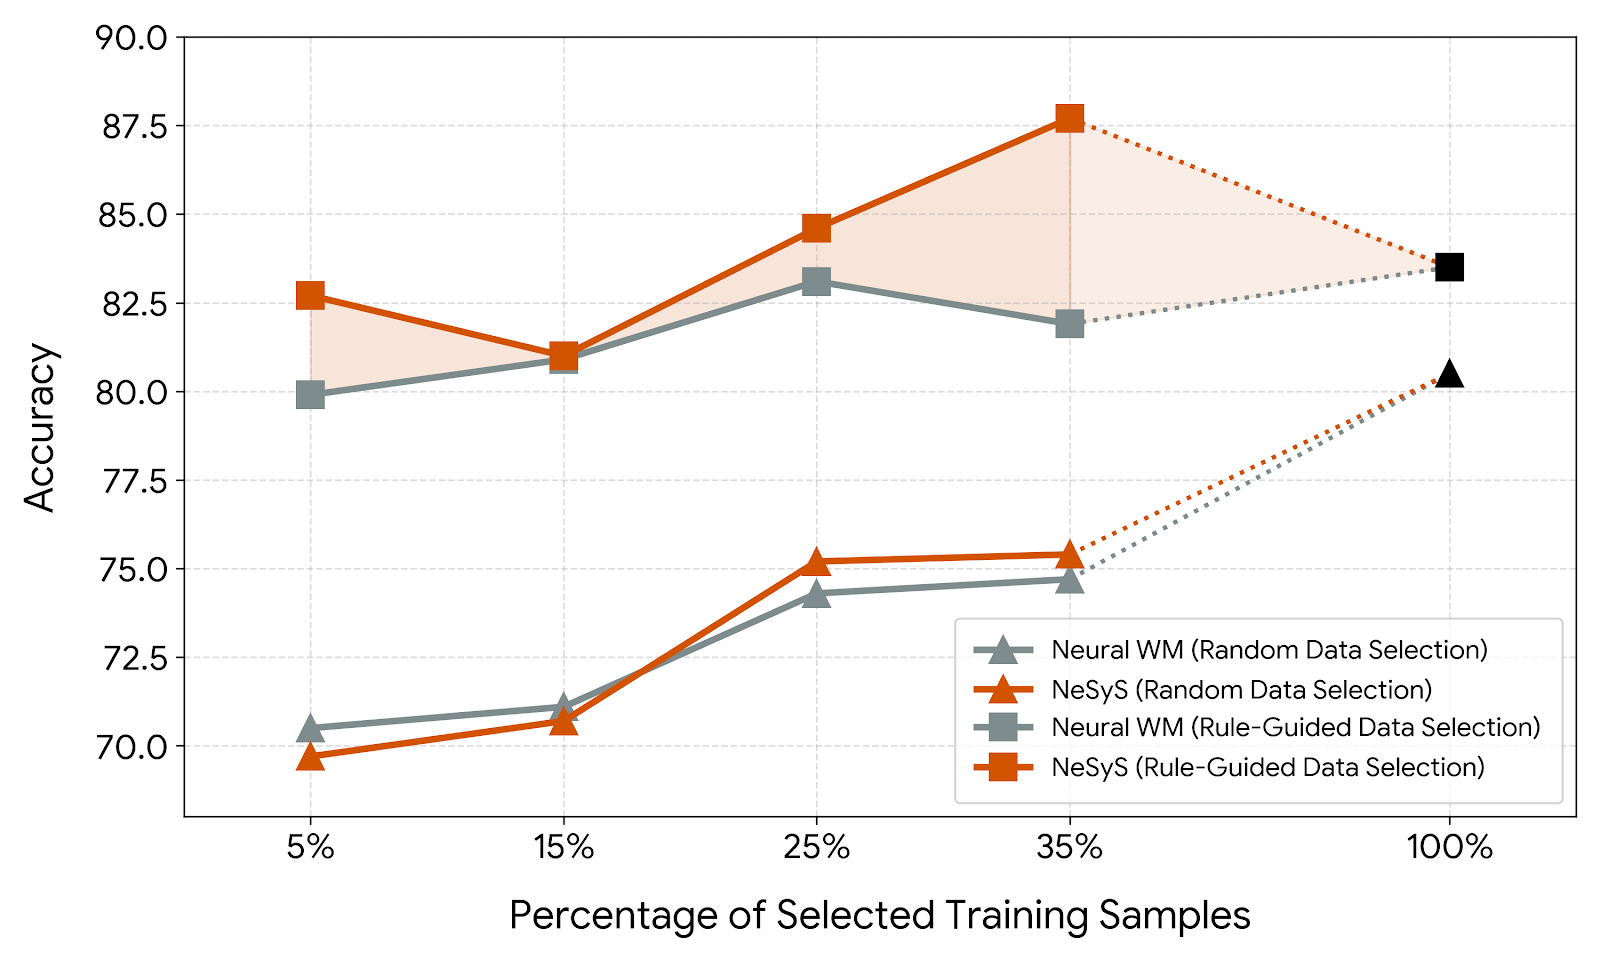
\includegraphics[width=\columnwidth]{images/random_vs_rule_filtering.png}
\caption{Comparing rule-guided data selection (ours) vs. random data selection under different training budgets on Plancraft. The backbone model is Llama-3.2-1B-Instruct. The shadow in the figure highlights the performance gain of our strategy.}
\label{fig:random_vs_rule_filtering}
\end{figure}

\paragraph{Exploration of training a lightweight router.} 
Building on the neuro-symbolic synergy observed in our main experiments, we explored the potential of a routing mechanism to dynamically select the optimal configuration (i.e., Neural vs. Symbolic WM, phase 1 vs. phase 2 models, and the scaling factor $\gamma$). We compared a lightweight XGBoost router, trained on the development set, against an 'oracle' router that acts as a theoretical upper bound by always selecting the optimal parameters. As detailed in \cref{app:router}, the XGBoost router yielded marginal gains over the baseline \ours. However, the oracle router achieved near-perfect scores, indicating that while simple routing is insufficient, developing a more sophisticated selection mechanism remains a high-potential direction for future work.

\section{Conclusion} \label{sec:conclusion}
In this work, we introduced \ours, a novel framework that bridges the gap between the broad semantic reasoning of LLMs and the strict logical consistency required for rigorous world modeling. By treating executable symbolic rules as energy functions that directly modify the LLM's output distribution, our approach enforces deterministic constraints without relying on the model's variable instruction-following capabilities. Empirical results validate \ours' consistent effectiveness and efficiency across diverse domains and model scales. While our current implementation effectively combines neural and symbolic signals, our analysis suggests that more sophisticated, dynamic routing between these modules represents a high-potential direction for future work. %Ultimately, \ours establishes a scalable and data-efficient pathway for building agents that are both semantically flexible and logically robust. 


%Beyond performance gains, we also demonstrated the efficiency of \ours. Our rule-guided data selection strategy reveals that substantial portions of training data in interactive environments are redundant once simple logical behaviors are codified. By filtering out these rule-compliant examples, we allow the neural model to focus its capacity on learning complex, implicit dynamics. This strategy reduced training data requirements by approximately 50\% while consistently outperforming fully fine-tuned baselines.

%Empirical results across ScienceWorld, Webshop, and Plancraft validate that \ours is robust across diverse domains and model scales. While our current implementation effectively combines neural and symbolic signals, our analysis suggests that more sophisticated, dynamic routing between these modules represents a high-potential direction for future work. Ultimately, \ours establishes a scalable and data-efficient pathway for building agents that are both semantically flexible and logically robust.

\section*{Impact Statement}
This paper presents work whose goal is to advance the field of Machine
Learning. There are many potential societal consequences of our work, none of which we feel must be specifically highlighted here.

\bibliography{wm}
\bibliographystyle{icml2026}

\newpage
\appendix
\onecolumn
% \section{Rule Guided Data Selection vs Random Data Selection}\label{app:ablation}
% As discussed in \cref{sec:ablation}, we conduct an ablation study on the data selection methods. As is shown in \cref{fig:random_vs_rule_filtering}, Neural WMs trained with two data selection methods perform similar without symbolic rules, but rule-guided method consistently perform better when paired with Symbolic WM. Additionally, we observe that the performance of Neural WM keeps improving until using all the training samples, but this is not true for \ours. These two observations further prove the complementary strengths of Neural and Symbolic WM in our framework, and the effectiveness of the proposed rule-guided data selection mechanism. See \cref{app:ablation} for details.
% \begin{figure}[ht]
% \centering
% 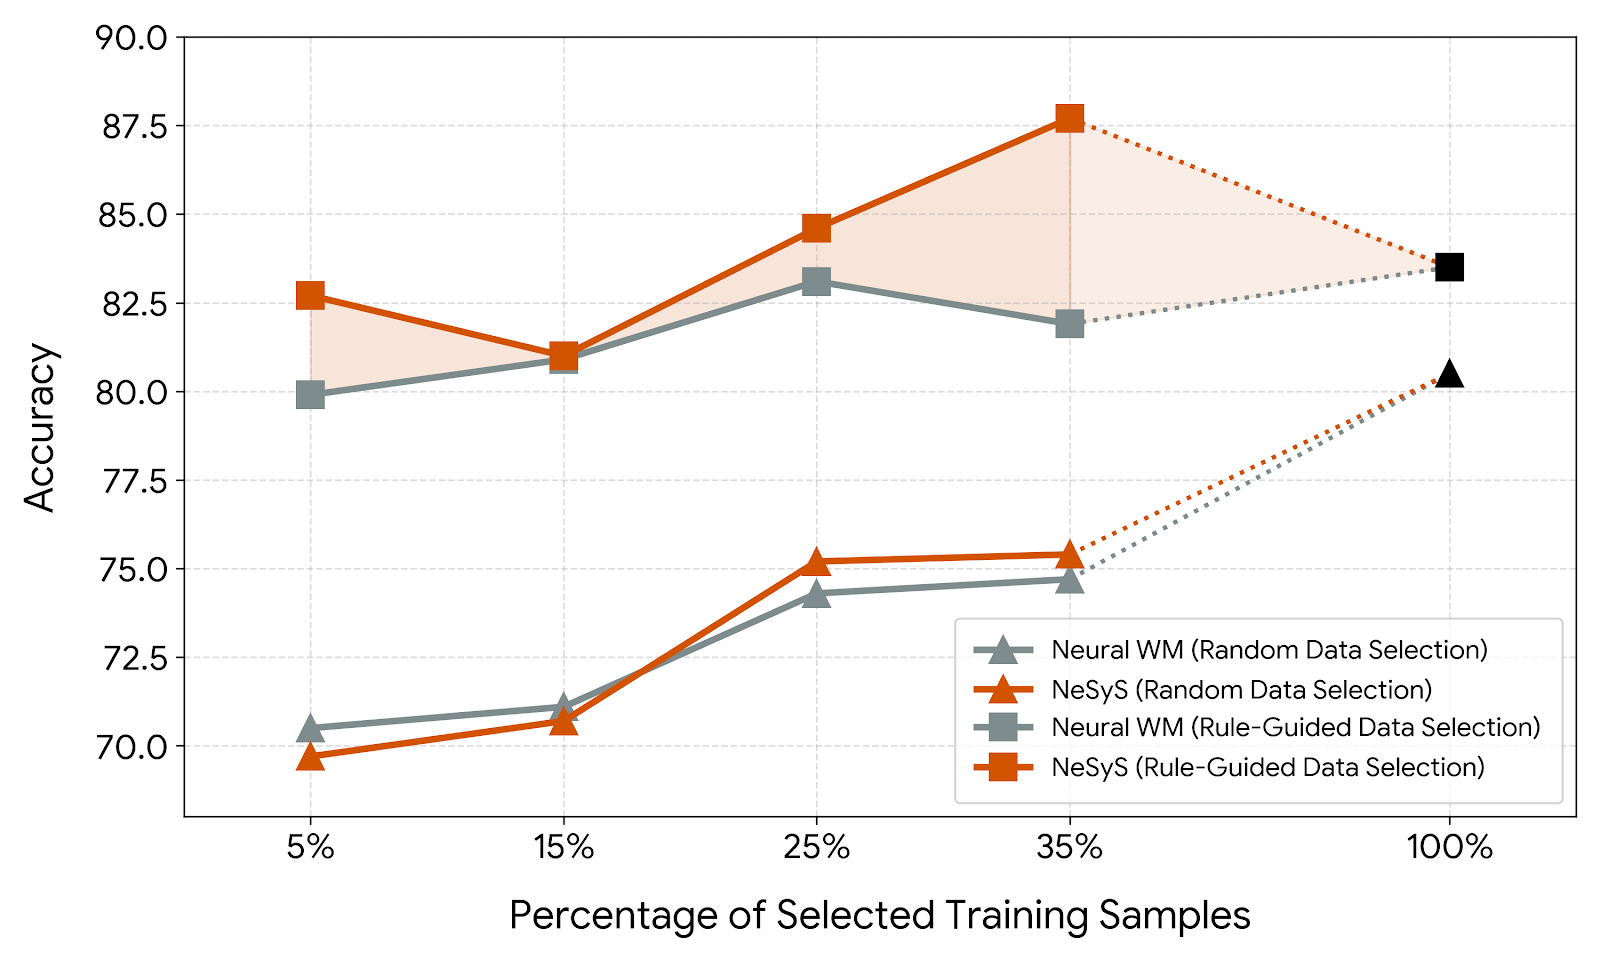
\includegraphics[width=0.7\linewidth]{images/random_vs_rule_filtering.png}
% \caption{Comparing rule-guided data selection (ours) vs. random data selection under different training budgets on Plancraft. The base model is Llama-3.2-1B-Instruct. The shadow in the figure highlights the performance gain of our strategy.}
% \label{fig:random_vs_rule_filtering}
% \end{figure}
\section{Evaluation Prompt}\label{app:prompt_eval}
When evaluating on ScienceWorld, we include recent trajectories and a memory of each visited location before the beginning of the trajectories, and ask for predicting the next observation, reward and difference of inventory. Here is the prompt we used:
\begin{tcolorbox}[
  title=Prompt used for Evaluating on ScienceWorld,
  colback=gray!5,
  colframe=black!50,
  fonttitle=\bfseries
]
\textbf{System:} You are a ScienceWorld transition model. Given the compressed history and ONE action, output exactly three lines in this order:\\
predicted\_observation: <text>\\
predicted\_reward: <float in [-1,1]>\\
predicted\_inventory\_diff: <one or more lines with '+ ' or '- ' prefixes only>
Do not output any additional text. \\[0.5em]
\textbf{User:} Task Description: \{task description\}\\
Memory (last look-around per visited location): \{memory\}\\
action: \{$a_k$\}\\
observation: \{$s_{k+1}$\}\\
reward: \{$r_{k}$\}\\
\ldots \\
current\_step\_action: \{$a_t$\}\\
\end{tcolorbox}

Here is the prompt we used for evaluating on Webshop:
\begin{tcolorbox}[
  title=Prompt used for Evaluating on Webshop,
  colback=gray!5,
  colframe=black!50,
  fonttitle=\bfseries
]
\textbf{System:} You are a transition model for the WebShop text environment. \\
Given the current page text (state) and the action taken, predict the next page text. \\
Your answer must be ONLY the next state's text, with no extra commentary. \\[0.5em]
\textbf{User:} Current state (page text): \{state\} \\
Action taken: \{$a_t$\}\\
Question: What is the next state's page text? Answer with ONLY the next state's text. 
\end{tcolorbox}

Here is the prompt we used for evaluating on Plancraft:
\begin{tcolorbox}[
  title=Prompt used for Evaluating on Plancraft,
  colback=gray!5,
  colframe=black!50,
  fonttitle=\bfseries
]
\textbf{System:} You are a Minecraft transition model. Given a current state and ONE action, return the next state text in the exact format used by the data (same headers and lists). Do not output actions. Enforce environment rules: cannot move/smelt into [0]; crafting outputs appear at [0] and must be moved to an inventory slot to complete. Output only the next state text. \\[0.5em]
\textbf{User:} \{state\} \\
Action: \{$a_t$\}
\end{tcolorbox}

\section{Rule induction Prompts}\label{app:prompt_rule_induction}
Here are the prompt we used for rule inductions for each environment. Example programs are omitted for clarity, they are essentially python programs that implement the example rules and can be found in our published code.

\begin{tcolorbox}[
  title=Rule induction for Webshop,
  colback=gray!5,
  colframe=black!50,
  fonttitle=\bfseries,
  breakable
]
\textbf{User:}

Analyze the following WebShop transition model error cases and summarize one actionable improvement rule. Follow these guidelines:

\textbf{[Error Cases]} \\
\{cases\}

\textbf{[WebShop Format]}
\begin{itemize}
  \item The state text is the current WebShop page content.
  \item The action is an environment action such as:
  \begin{itemize}
    \item \texttt{click[buy now]}
    \item \texttt{click[< prev]}
    \item \texttt{search[...]}
  \end{itemize}
  \item The choice is a candidate next state or a terminal token: Success or Fail.
\end{itemize}

\textbf{[Analysis Requirements]}
\begin{enumerate}
  \item Identify shared action types across cases.
  \item Infer what the correct next page or terminal result should be.
  \item Formulate one generalizable and checkable rule returning a score in $[-1,1]$.
  \item Apply the rule only when its conditions match; otherwise return 0.0.
  \item Phrase the rule after \#\#\# Rule \#\#\#.
  \item Write a Python program after \#\#\# Program \#\#\#.
\end{enumerate}

\textbf{[Example Rules and Programs]}

1) Example rule (Buy Now missing => Fail): If action is exactly click[buy now] but the current page text does NOT contain a Buy Now button,
   then the correct terminal result is Fail. Return 1 if choice is Fail and -1 otherwise.

Example Program: (Omitted)

2) Example rule (< Prev => back to results): If action is click[< prev] and the current page text contains a < Prev button,
   then the next page is usually a search results list page that contains 'Total results' and a 'Next >' button.

Example Program: (Omitted)
\end{tcolorbox}

\begin{tcolorbox}[
  title=Rule induction on Plancraft,
  colback=gray!5,
  colframe=black!50,
  fonttitle=\bfseries,
  breakable
]
\textbf{User:}

Analyze the following model error cases and summarize one actionable improvement rule. Follow these guidelines:

\textbf{[Error Cases]} \\
\{cases\}

\textbf{[Analysis Requirements]}
\begin{enumerate}
  \item Try to find patterns in the questions. What do they have in common? Are the actions of the same type? Do the states share similarities?
  \item Try to find patterns in the correct answers. What are their shared characteristics?
  \item Try to find patterns in the incorrect answers. What makes them incorrect?
  \item Formulate one generalizable rule for the presented error cases. The rule should be detailed enough to be programmed and used to score each candidate choice. It should apply only when the shared patterns are observed, encouraging correct patterns and discouraging incorrect ones.
  \item If a detailed rule cannot be found for all error cases, describe a rule for a subset rather than being vague.
  \item Phrase the rule after \#\#\# Rule \#\#\#.
  \item Write a Python program after \#\#\# Program \#\#\#. The program should define a function rule\_reward(state, action, choice) that returns a float in $[-1,1]$, indicating how likely the choice is correct.
\end{enumerate}

\textbf{[Example Rule and Programs]}

\textbf{Example rule 1.} For a move action "move: from [I?] to [A/B/C?] with quantity q", the next state should reflect only the intended move. Penalize choices that change unrelated item counts.

\textbf{Example program:} (Omitted)

\textbf{Example rule 2.} For illegal actions other than move or smelt, the next state should not change.

\textbf{Example program:} (Omitted)

\end{tcolorbox}

\begin{tcolorbox}[
  title=Rule induction for ScienceWorld,
  colback=gray!5,
  colframe=black!50,
  fonttitle=\bfseries,
  breakable
]
\textbf{User:}

Analyze the following ScienceWorld model error cases and summarize one actionable improvement rule. Follow these guidelines:

\textbf{[Error Cases]} \\
\{cases\}

\textbf{[ScienceWorld Format]}
\begin{itemize}
  \item The state text is a compressed history including task description, optional memory, per-step history (action, observation, reward), and inventory or inventory\_diff snippets. It ends with current\_step\_action: <action>.
  \item The choice must contain exactly the following lines (order fixed):
  \begin{itemize}
    \item predicted\_observation: <text>
    \item predicted\_reward: <float in [-1,1]>
    \item predicted\_inventory\_diff: <zero or more +/- lines>
  \end{itemize}
\end{itemize}

\textbf{[Analysis Requirements]}
\begin{enumerate}
  \item Identify common action types (e.g., open X, pick up Y, use thermometer on Z).
  \item Infer what consistent predictions should look like for these actions.
  \item Design a rule that checks these consistencies by parsing the choice and, if needed, extracting the current action from the state.
  \item The rule should be specific and return a score in $[-1,1]$.
  \item Phrase the rule after \#\#\# Rule \#\#\#.
  \item Write a Python program after \#\#\# Program \#\#\# defining \texttt{rule\_reward(state, action, choice)}.
\end{enumerate}

\textbf{[Example Rules and Programs]}

1)Example rule (Pick up): If action starts with 'pick up <obj>', then:
   - predicted\_observation contains 'You move the <obj> to the inventory.'
   - predicted\_inventory\_diff contains a line starting with '+ ' and mentioning <obj>.
   
Example Program: (Omitted)

2) Example rule (Open): If action matches 'open <obj>', require:
   - predicted\_observation contains 'The <obj> is now open.' (or 'already open')
   - predicted\_inventory\_diff is empty or contains no changes

Example Program: (Omitted)

3) Example rule (Thermometer): If action contains 'use thermometer' and 'on <target>', then:
   - predicted\_observation contains 'the thermometer measures a temperature of'
   - predicted\_inventory\_diff should be empty

Example Program: (Omitted)
\end{tcolorbox}
We use the following prompt for reflection in rule induction:
\begin{tcolorbox}[
  title=Prompt for reflection in rule induction,
  colback=gray!5,
  colframe=black!50,
  fonttitle=\bfseries,
  breakable
]
\textbf{User:}

The following rule is causing negative impacts on some questions that were originally answered correctly. Please refine the rule to avoid these negative impacts while maintaining its beneficial effects.

\textbf{[Current Rule Description]} \\
\{rule\_description\}

\textbf{[Current Rule Program]}
\{current\_rule\}

\textbf{[Negative Impact Cases]}
\{negative\_impacted cases\}

\textbf{[Refinement Requirements]}
\begin{enumerate}
  \item Analyze why the current rule is causing originally correct answers to become wrong.
  \item Identify the specific conditions or patterns responsible for the negative impact.
  \item Refine the rule to be more precise and avoid these false positives.
  \item Maintain the beneficial effects the rule was designed to achieve.
  \item Make the refined rule more conservative to avoid breaking correct predictions.
  \item Write the refined rule after \#\#\# Rule \#\#\#.
  \item Write the refined Python program after \#\#\# Program \#\#\#. The program should define rule\_reward(state, action, choice) and return a float in $[-1,1]$.
\end{enumerate}

\textbf{[Focus Areas for Refinement]}
\begin{itemize}
  \item Add more specific conditions to prevent false positives.
  \item Consider edge cases that may be incorrectly handled.
  \item Make the rule more conservative in its judgments.
  \item Add additional validation checks before applying penalties or rewards.
\end{itemize}
\end{tcolorbox}

\section{Clustering Details}\label{app:clustering}
We cluster the error cases based on the embeddings of the following part of the case respectively:
\begin{itemize}
    \item question
    \item correct answer
    \item wrongly selected answer
    \item action
    \item task name
\end{itemize}
To convert text to embedding, we first concatenate a tf-idf embedding of the selected text with the embedding generated by \texttt{all-MiniLM-L6-v2} from sentence transformers~\citep{reimers-2019-sentence-bert}. We reduce the dimension to 50 with a truncated SVD, then to 5 with a UMAP. We use the OPTICS algorithm with min samples=3, xi=0.05 and min cluster size=0.1 for clustering. 

\section{Router Training}\label{app:router}
We train the XGBoost router with the following features:
\begin{itemize}
    \item Scores provided by each rule
    \item Logprob of each options provided by the base Neural WM
    \item Length of the question
    \item Length of the action
    \item task name
\end{itemize}
We try all combinations of the features and select the model with best dev set accuracy. We use a fixed set of hyperparameters: n estimators=2500, max depth=6, learning rate=0.01.

The detailed result is shown in \cref{tab:router}. The analysis can be found at \cref{sec:ablation}.
\begin{table}[ht]
  \caption{Performance of an oracle router and an actually trained XGBoost router.}
  \label{tab:router}
  \centering
  \begin{tabular}{lcccc}
    \toprule
    \cmidrule(r){1-2}
    Model & ScienceWorld & Webshop & Plancraft & Average\\
    \midrule
    \multicolumn{5}{c}{\bf Llama3.2-1B} \\
    \midrule
    \ours & 68.3& 92.2& 87.7 & 82.7 \\
    XGBoost router & 68.7 & 92.4 &88.6 & 83.2\\    
    Oracle router & 82.9 & 94.3 & 95.8 & 91.0 \\
    \midrule
    \multicolumn{5}{c}{\bf Qwen3-4B} \\
    \midrule
    \ours & 71.0& 92.6& 88.4& 84.0 \\
    XGBoost router & 71.0 & 91.3&91.5 & 84.6\\   
    Oracle router & 84.2 & 99.9 & 98.2 & 94.1 \\
    \bottomrule
  \end{tabular}
\end{table}
\section{Benchmark Creation Details}\label{app:data-collection}
As discussed in \cref{sec:exp_setup}, we create the benchmarks based on the official expert trajectories provided by the environment. Here we enclose the details for each environment.

For ScienceWorld, we sample at most 50 dev/test variations from each pre-defined task (there are 30 predefined tasks in the environment), and at most 5 positions from each variation. We create one question at each position. 

For Webshop, we do a random 90:5:5 train:dev:test split on the provided trajectories. We use every time step in the dev/test trajectories to create a question. Since all the trajectories end up successfully buying the desired item, we randomly select middle positions of each trajectory and insert a ``click[buy now]'' action, which will result in a "Fail" state. Similar operation is performed on the training set.

For Plancraft, we sample at most 6 steps from each provided dev/test trajectories. We enriched the training trajectory by 
\begin{itemize}
    \item Using side products in existing trajectory as goal and truncate the trajectory up to that position.
    \item Starting from the existing setups and generating new trajectories by looping through all possible recipes.
    \item Modifying the starting inventory of existing trajectories by removing a required ingredient or swapping it with a similar item.
\end{itemize}

After we sample the questions and the correct answers, we use \texttt{Llama-3.2-1b-instruct} to answer questions and use the wrong ones as the distractors.

\section{Rigorous Definition of POMDP}\label{app:pomdp}
In \cref{sec:problem}, we defined the problem in a informal way for better understanding. Here we provide the rigorous definition of the POMDP problem we are studying. The problem is usually written as $\mathcal{M} = (S, A, T, R, \Omega, O)$, where $S$ denotes the latent state space, $A$ the action space,
$T : S \times A \to \Delta(S)$ the transition kernel, $R : S \times A \to \mathbb{R}$ the reward function, $\Omega$ the observation space, and $O : S \times A \to \Delta(\Omega)$ the observation kernel. In this work, both actions $a_t \in A$ and observations $\omega_t \in \Omega$ are represented as natural-language strings.

A \emph{world model} is defined as a predictive model that estimates the next observation $\omega_t$ and reward $r_t$ conditioned on the current action $a_t$
and belief state $b_t$. Following prior LLM-based agent work, we approximate the belief state by a textual context constructed from the task description $g$ and a truncated history of recent observations, actions, and rewards that fit within the model’s context window.
\end{document}
